\section{Introduction}
Agilefant is an open source tool for task and requirement management for agile 
software development. It is provided as an open-source version and a hosted 
version. The hosted version comprises more and better features in comparison to 
the open-source version.

Agilefant has approximately 10,000 users worldwide, and according to the 
customer, the number of registered users increases every day. 
 
Agilefant is a very powerful tool for requirement management but currently it 
is too detailed to be used on mobile devices (small screens). The customer 
wishes that the users of Agilefant could use its the most important functions 
using their mobile phones and tablets. Agilefant's main competitors are already 
providing mobile applications, so it is crucial to Agilefant to response for 
this. Therefore, the goal of our team is to develop a mobile application that 
works along the hosted version of Agilefant and can be used on both smart 
phones and tables.

\subsection{Vision}

Agilefant's vision is to become the leading provider of agile backlog management tools.

\section{Stakeholders and staffing}

The project contains several stakeholders, which are presented in 
Figure~\ref{fig:stakeholders}. The stakeholders are divided into four groups: the customer 
(Agilefant), the student group, the teaching personnel in Aalto University, and teaching 
personnel in University of Victoria. Arrows in the figure present the direction of main 
communication.

\begin{figure}[H]
\centering
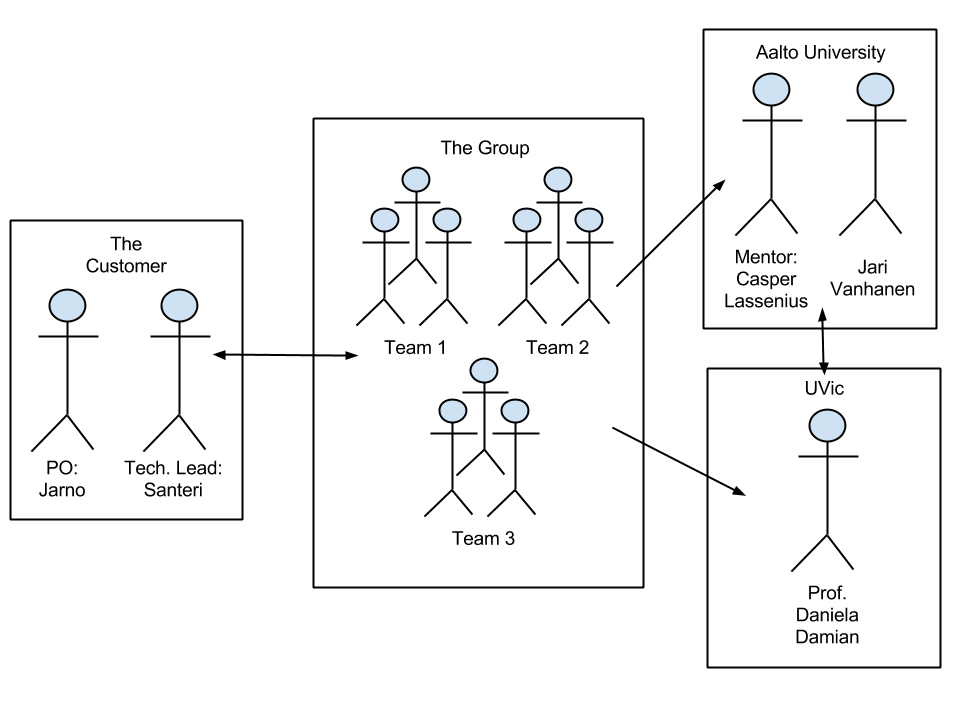
\includegraphics[width=1\textwidth]{imgs/stakeholders.png}
\caption{Stakeholders of the project}
\label{fig:stakeholders}
\end{figure}

\subsection{The Team}

Here we are only listing the role, name, email, responsibilities and an 
assistant role of each team member. We have a document with everyone's personal 
informations such as email, phone number and Github name, but we won't publish 
those informations excluding email.

The group's email is mobilefant\#agilefant.org.

We have several roles and one person can have several roles. The primary roles are bolded. The roles are:

\begin{itemize}
\item Scrum Master = SM
\item Project Manager = PM
\item Lead Architect = AR
\item Quality Assurance = QA
\item Requirements Engineering = RE
\item Developer = Dev
\end{itemize}

\begin{table}[H]
\center
\resizebox{\textwidth}{!}{
\begin{tabular}{|p{1.8cm}|p{3cm}|p{4.1cm}|p{4.1cm}|p{1.8cm}|} 
	
\hline % The line on top of the table
\textbf{Role} & \textbf{Name} & \textbf{Email} & \textbf{Responsibilities} & 
\textbf{Assistant role} \\ 
\hline 
\textbf{SM, PM}, RE & Benjamin Behm & benjamin.behm\#aalto.fi & Organizing the 
work, removing impediments, documenting, process supervising, eliciting 
requirements & - \\ 
\hline
\textbf{AR}, RE & Harri Lampi & harri.lampi\#aalto.fi & Architectural design, 
eliciting requirements, coding, UI design & - \\ 
\hline
\textbf{QA}, RE & Matias Kuusela & matias.kuusela\#aalto.fi & Quality assurance, eliciting requirements, UI design & -\\ 
\hline
\textbf{Dev} & Miro Vilkki & miro.vilkki\#aalto.fi & End-to-end development & \\
\hline
\textbf{Dev} & Rolle Saarinen & rolle.saarinen\#aalto.fi & End-to-end development & \\
\hline
\textbf{Dev} & Janne Gröndahl & janne.grondahl\#aalto.fi & End-to-end development & QA\\
\hline
\textbf{Dev} & Janne Kajovuori & janne.kajovuori\#aalto.fi & End-to-end development, documenting, UI design & PM\\
\hline
\textbf{Dev} & Joakim Kronqvist & joakim.kronqvist\#aalto.fi & End-to-end development & AR\\
\hline

\end{tabular} % for really simple tables, you can just use tabular
}
\caption{The team}
\label{table:Team}
\end{table}

NB! Each developer should act as an assistant to some of the SE experts in 
order to get a broader view of the project.

\subsection{Mentor}

\begin{table}[H]
\center
\begin{tabular}{|p{2cm}|p{3.8cm}|p{4.1cm}|} 

\hline 
\textbf{Role} & \textbf{Name} & \textbf{Email} \\ 
\hline
Mentor & Casper Lassenius & casper.lassenius\#aalto.fi \\
\hline
\end{tabular}
\caption{Mentor}
\label{table:Mentor}
\end{table}

\subsection{Customer}

\begin{table}[H]
\center
\begin{tabular}{|p{2cm}|p{3.8cm}|p{4.1cm}|} 
	
\hline 
\textbf{Role} & \textbf{Name} & \textbf{Email}\\ 
\hline
Product owner & Jarno Vähäniitty & jarno\#agilefant.org\\
\hline
Tech. Lead & Santeri Korri & santeri\#agilefant.org\\
\hline
\end{tabular} 
\caption{Customer representatives}
\label{table:Customer}
\end{table}



\section{The Goals}
\subsection{Project goals}

The main goal is to develop a reliable mobile application for Agilefant that
contains the main functionalities of its cloud version and fulfil customer's
vision of the product. Furthermore, the goal is that everyone's personal goals
will be reached and the course has been an educational experience. In order to
support these learning goals, tasks are tried to assign to people so that the
course help them to learn what they want to learn. Other high level goals are
identified, and these are presented in Table~\ref{table:Projectgoals}.

\begin{table}[H]
\center
\resizebox{\textwidth}{!}{
\begin{tabular}{|p{0.5cm}|p{6.5cm}|p{6.5cm}|} 

\hline 
\centering \textbf{\#} & \textbf{Goal} & \textbf{Verification Criteria} \\ 
\hline

\centering 1 & To produce high customer satisfaction & Customer's personal opinion about the delivered product. \\
\hline

\centering 2 & To build a limited set of key use cases & Architecturally sound, 
clear implementation and testable. \\
\hline

\centering 3 & The product will be released after the project & Whether the customer release the product or not. \\
\hline

\centering 4 & To get grade 5 & The grade will be visible in transcript of records or the course personnel has verified the grade. \\
\hline

\centering 5 & To win the quality award & Our group has selected as the best group at the end of the course. \\
\hline

\end{tabular}
}
\caption{Project goals in the priority order}
\label{table:Projectgoals}
\end{table}


\subsection{Personal goals}

As we are here learning new things, we should focus to learn things we are interested in. Thus, it is important that everyone tells theirs interests aloud and points out what they would like to learn during this course. 

If a developer is going to take this course second time later and has a preferable role in his mind, it is really recommendable that he takes some responsibility of that manager role.

Personal learning goals can be found in Google Docs: 
\href{https://docs.google.com/spreadsheet/ccc?key=0Ahu59q_GwtcedHJZdjQ1RWROZFYxa
0RTcWp3MkJkTnc&usp=sharing}{Learning Goals}

\section{Resources}
\subsection{Personnel}

Each member must invest ``credits * 27 hours - 15 hours in the project''.

\href{https://docs.google.com/spreadsheet/ccc?key=0Ahu59q_GwtcedHI3MnJQM0NWZS11a
GxFTzFZeVEyQVE&usp=sharing}{Link} to the time allocation page. Everyone should 
mark how much time he/she is going to use per a week to the table.

\subsection{Material}

We need mobile phones to test the application. The customer has promised to 
deliver some test phones, but a wide range of different phones with different 
platforms cannot be guaranteed. In this reason we will use our own mobile phones for testing.

The CSE department borrows three desktop computers 
to our group with Ubuntu 12.04 installed. These computers have been set up 
to our team room A243.

The room (A243) will be shared with an another project group (\#15 - 
TrafficSense) so we need to schedule the usage of the room with them. The idea 
will be that both teams will have specific days and hours the room is 
exclusively reserved for them. At other times, everyone could use the room.

A development environment can be downloaded from Internet if needed. Eclipse is 
an open-source and free to download, and the project manager has a JetBrain's 
Classroom License, so that IntelliJ IDEA Ultimate can be used during the course.

\section{Work practices}

In this section we describe what working practices we have planned to use on this course. Each group member should understand what practices are used and how to adopt them properly in order to work efficiently.

\subsection{Practices}
\subsubsection{Iterative development}

We are working iteratively during the course. The idea is to build the product 
incrementally and iteratively. We will be using an agile software development 
method called Scrum. Its focus is to provide guidelines that enable flexible 
way of working and allow the development team to react to changes in 
requirements faster than traditional development frameworks.

The course is divided into three phases (Planning, Implementation 1 and 
Implementation 2). We don't emphasize these phases as we have planned to have two sprints before the Christmas and seven sprints after the Christmas. Because of the exam week on week 8, we have one sprint of three weeks whereas the other sprints are two weeks. 

We will be following the scrum practices meaning that we will keep sprint planning, sprint review and sprint retrospective sessions in every sprint.

\begin{figure}[H]
\centering
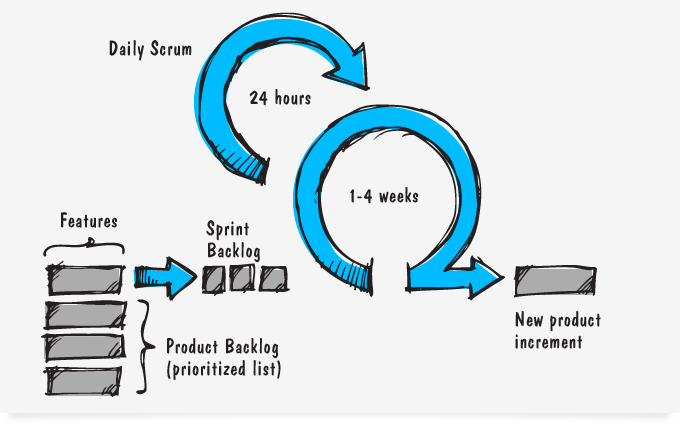
\includegraphics[width=1\textwidth]{imgs/scrum_process_en.png}
\caption{Scrum process}
\label{fig:scrum}
\end{figure}

\subsubsection{Sprint planning}

Sprint planning session will be divided into two parts. The content of the 
sprint planning is presented in Table~\ref{table:Sprintplanning}. The project management has responsible for arranging sprint planning sessions.

The sprint planning session will be held using Google Hangout so that The Finns are located in their team room in Finland and the Canadiens are located in their class room in Vancouver, Canada.

\begin{table}[H]
\center
\resizebox{\textwidth}{!}{
\begin{tabular}{|p{1cm}|p{2cm}|p{5cm}|p{4cm}|} 
	
\hline 
\textbf{Part} & \textbf{Duration} & \textbf{Description} & 
\textbf{Participants} \\ 
\hline
1 & 1h & The product owner presents the prioritized product backlog, so that 
the teams would understand what should be done during a following sprint. The 
product owner is there for answering any questions the teams would like to ask 
relating to the user stories and tasks. Then the teams select items from the 
product backlog to the sprint backlog based on their knowledge of how much work 
they are capable of doing during a sprint. Sprint goal is agreed in this part. 
& Product owner, members of each team \\
\hline
2 & 2h & Teams are separated to plan how the chosen work will be done during 
the sprint. Users stories will be assigned to team members. User stories are 
split into tasks and the required time per a task is estimated by a person the 
task was assigned to. In this meeting, the team can start design the system so 
that they are able to convert the backlog items into a working software 
increment. & Team members \\
\hline
\end{tabular}
}
\caption{The content of a sprint planning}
\label{table:Sprintplanning}
\end{table}

In a sprint planning session (excluding sprint 1), stories are estimated using 
story points following the pattern of fibonacci numbers. Story points are not directly relating to possible time needed to finish a story but rather describe their 

 Possible 
story points are listed below with approximate time:
\begin{description*}
\item[1]
\item[2]
\item[3]
\item[5]
\item[10]
\end{description*}
	
If the story is estimated to be larger than 10 story points, it can be seen as 
an epic and should be split to smaller stories so that it can be finished 
during the sprint.

The customer said we should not have larger stories than 10 points.

\subsubsection{Documenting}

All course documents need to be public and available for everyone. The course 
personnel and customer should be able to follow the progress of the project by 
seeing our documentation. In addition, the change log of each documents 
documentation should be visible so that changes are easily seen.

The group's web page is located in 
\href{https://github.com/phyper/mobilefant-documentation/wiki}{Github}. That works as a base for links to actual documents.

The SE trio is responsible for writing mandatory course documentation. 
Developers can help to write documents based on their interests. Their effort 
is preferable at least when planning the architecture and eliciting 
requirements from the customer. 

\subsubsection{Risk management}

Trio held a risk management session together with one developer. The session was held in the middle of the first sprint and it took 30 minutes. During the session we identified several potential risks. When these risks were identified, we estimated the probability and severity of each risk and discussed a little bit how to minimize the occurrence of these risks. 

The risk log is maintained regularly by the SE trio. At the end of each sprint the log is review and updated.

\subsubsection{Time tracking}

The group's time tracking will be applied in Agilefant. The group should follow 
these time tracking practices:
\begin{itemize}
\item Each group member should enter their own hours by themselves to the 
Agilefant.
\item Hours are logged directly to the story or more preferably to the task 
after the work is done. 
\item Hours should be logged before leaving the office
\end{itemize}

Agilefant provides burndown charts that are used to follow the project's progress. Burndown charts tell also whether estimated hours are correlating with actual hours. That helps the group to shape its task estimation.

As the group is logging spent effort to the Agilefant, the customer is able to follow whether the group is working as promised. 

\begin{figure}[H]
\centering
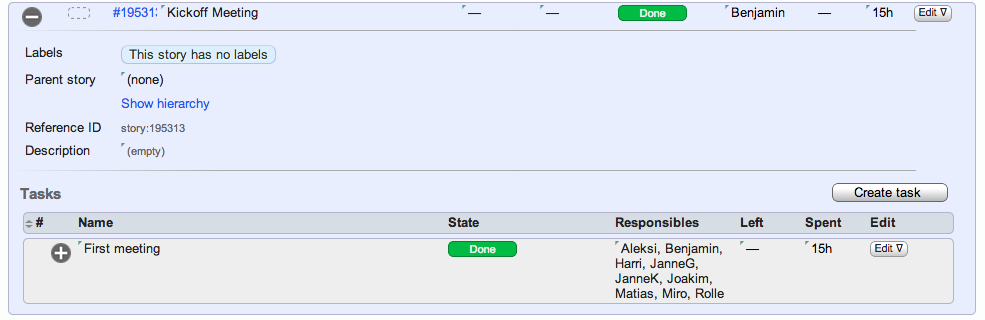
\includegraphics[width=1\textwidth]{imgs/spenteffort1.png}
\caption{Story and task with spent effort}
\label{fig:spenteffort1}
\end{figure}


\begin{figure}[H]
\centering
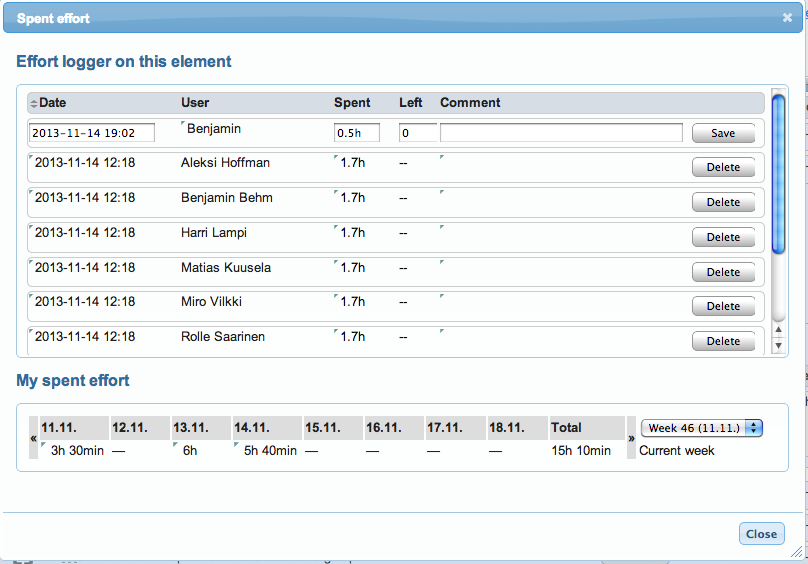
\includegraphics[width=1\textwidth]{imgs/spenteffort2.png}
\caption{Log spent effort}
\label{fig:spenteffort2}
\end{figure}

When the course is over, credits will be given based on the hours logged to the 
Agilefant (+ hours spent on lectures). The view shown in 
Figure~\ref{fig:totalhours} can be found in Timesheets where user needs to 
select backlog(s), interval and user(s) to generate the timesheet where used 
hours are listed.

\begin{figure}[H]
\centering
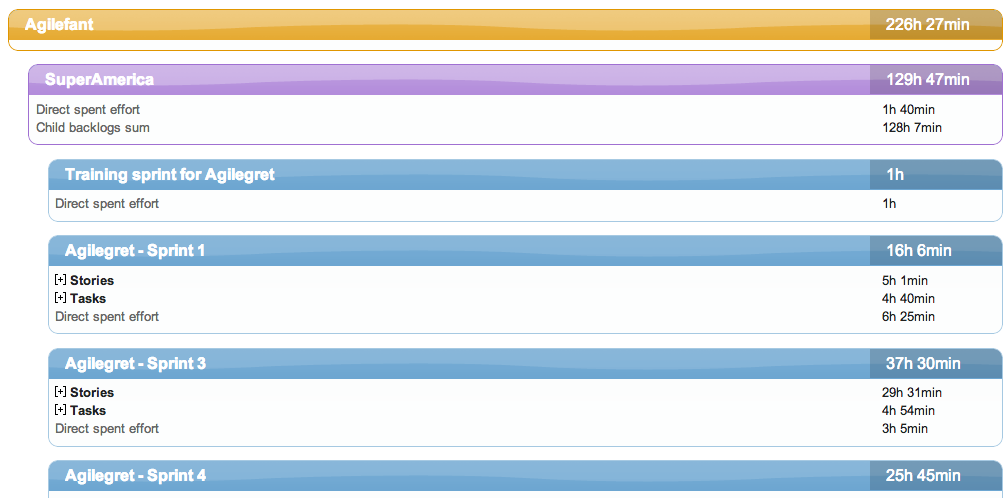
\includegraphics[width=1\textwidth]{imgs/totalhours.png}
\caption{Total used hours}
\label{fig:totalhours}
\end{figure}

\subsubsection{Communication}

Team will keep a daily standup meeting every time they gather together to work. 
The daily standup will be a short, 15-minute time-boxed meeting where team 
members synchronize their activities. In this meeting, people will tell, in 
turn, three things: What they have done since last daily meeting, what they 
will do before the next meeting, and what obstacles are in the way.  

The product manager will propose if the team could use Flowdock as the main 
communication tool. Aalto provides 180 days license for that.

Google Hangout is proposed to be used for communication with off-site team 
members.

In very urgent situations phone calls or text messaging can be used, but 
primary the group is using tools mentioned above.

\subsubsection{Defect tracking}

For defect tracking we are using Github's
\href{https://github.com/soberit/mobilefant/issues?state=open}{Issues}
functionality. It informs us immediately when new issues are created. Issues are also posted on our Flowdock stream from where everyone is able see them.

\subsubsection{Version control}

All code should be located in the version control system.
Agilefant uses Git (and Github) so we are also going to use 
them.

We have a private repository under Soberit organization. The repository is named as \href{https://github.com/soberit/mobilefant}{Mobilefant}.

We have decided to try out feature branching approach with a single repository. In feature branching each feature is developed using a separate 
branch in the version control system. This means that every time 
a developer starts a new feature, he/she will create a new 
branch for that, and after the feature is ready, the feature 
branch will be merged to the main branch. The main branch should 
contain only working code, which is verified by compiling the 
code and running the test. All tests should pass.

We have to be sure everyone understands how to use Github in order not to mess the whole repository as everyone has privileges to push anything into master.

We have defined a general git workflow. It can be found \href{https://docs.google.com/document/d/1wAih0JzkrZ4ySUZ_MO-F8MvGkPXKHicYbG1972Sxo2w/edit?usp=sharing}{here}.

\subsubsection{Process improvement}

A retrospective is arranged at the end of each sprint. The goal of having 
regular retrospectives is to improve the process and avoid roadblocks in 
development process.

For retrospectives, we are using \href{http://wirca.soberit.hut.fi/prod/}{ARCA-tool} developed in Aalto University. It's a tool that helps us to keep better retrospective meetings and analyze root cause of problems. In this way, these meetings can be more productive and less time will be wasted.

In general the ideas that are generated during a retrospective meeting are divided into two categories: what went well and what could be improved. 

The retrospective meeting is time-boxed to one hour (this depends on how much time 
Canadians have). We have to have enough time to sit down and discuss about the 
past sprint, otherwise there is no reason to keep this kind of meetings. 

The retrospective contains three phases:

\begin{enumerate}
\item First, everyone enters problems to ARCA-tool.
\item Second, the entered problems are discussed together.
\item Third, everyone enters underlying causes to the problems identified earlier.
\item Fourth, causes are discussed and additional causes are added if needed.
\item Fifth, findings are summarized at the end of the meeting.
\end{enumerate}

\subsubsection{Requirement engineering}

Requirement eliciting is up to the SE trio, but other team members can also 
participate in the eliciting process.

Requirements are collected to Agilefant. 

The customer is responsible for prioritizing the product backlog that is located 
in Agilefant.

Requirements should be presented as a format of a user story. This format helps 
everyone to capture the who, what and why of a requirement. The template for a 
user story is following:

\begin{verbatim}
    As a <role>, I want <goal/desire> so that <benefit>.
\end{verbatim}

In a user story, the role and goal/desire are mandatory, but the benefit part is 
optional.

\subsubsection{Design}



\section{Phasing}

Tasks are not listed in this project plan, as they are listed and maintained in 
\href{https://cloud.agilefant.com/dev/}{Agilefant}.

\subsection{Schedule}

Our schedule is still an open question as we don't know how we are going to organize the first sprint in Canada. We have talked that it could be done in cooperation with the Finns, but on the other hand, it would be easier to them if they can practice scrum practices without distributed aspect.

Project manager and QA are going to Canada with the customer and mentor on 8.1.2014 - 20.1.2014. Their task is to help Canadian students to get in to the project by teaching them what Agilefant is and what processes we are using. This is a kind of kickoff session for them.

\begin{verbatim}
Sprint 1 (13.11.2013 - 27.11.2013)
Sprint 2 (27.11.2013 - 11.12.2013)
Christmas vacation
Sprint 3 (7.1.2014 - 
Sprint 4
Sprint 5
Sprint 6
Sprint 7
Sprint 8 (X.X.2014 - 9.4.2014) 
\end{verbatim}

\subsection{Sprint 1 Plan}

Goals:
\begin{itemize}
\item To understand Agilefant's vision
\item To have the main requirements from the Customer
\item To understand the used process
\item To understand the domain
\item To have a draft of UI using wireframes
\item To know required technologies
\item To know tools that are going to be used
\item Working place ready at A243 with a couple of work stations
\end{itemize}

\subsection{Sprint 2 Plan}

Goals:
\begin{itemize}
\item To have the development environment set up to everyone
\item To have everyone working with the code 
\item To have the code base ready 
\item To have the high-level architecture design ready
\item To have the wireframes ready
\end{itemize}

\noindent Deliverables:
\begin{itemize}
\item Project plan (no QA plan)
\item Progress report slides
\item Contract (one per a group)
\item Requirements document (except details of requirements)
\end{itemize}

\subsection{Sprint 3 Plan}

Goals:
\begin{itemize}
\item To get to know the Canadians students
\item To familiarize Canadians to used practices and processes
\item To form three distributed teams

\end{itemize}

\section{Risk log}

\begin{table}[H]
\center
\resizebox{\textwidth}{!}{
\begin{tabular}{|p{0.5cm}|p{3cm}|p{1cm}|p{1.5cm}|p{4cm}|p{4cm}|p{1cm}|} 
	
\hline % The line on top of the table
\textbf{ID} & \textbf{Risk} & \textbf{Prob.} & \textbf{Sev.} & \textbf{Effects} 
& \textbf{Controlling actions} & \textbf{Resp.} \\ 
\hline

1 &
A developer quits in the middle of the project. &
2 &
3 & 
Some knowledge is lost. Project scope must be decreased. &
Taking care of good team spirit. Using pair programming. &
PM / All \\
\hline

2 & 
Adapting with Scrum practices is harder than expected. & 
2 & 
2 & 
Productivity is lower than assumed and stories cannot be finished on time. & 
Providing enough training. & 
PM \\
\hline

3 &
The team could not build a code base that is wide enough to divide development 
tasks among three teams on January. &
3 &
3 &
All developers cannot start development right away, but need to wait until the 
code base is ready. The project scope must be decreased. &
Architectural design needs to be started asap. Team members should start coding 
small features asap to get familiar with technologies. &
AR \\
\hline

4 &
The customer has to leave the CS-building on January, 2014. &
2 &
3 &
Getting feedback takes longer and the amount of face-to-face meetings decreases. 
&
To generate a backup plan of how stay contacted with the customer. &
PM / Customer \\
\hline

5 &
Merge conflicts when all have privileges to push staff to master &
3 &
3 &
Lots of effort have to put to resolve the problems. &
Git training should be provided to everyone if needed. &
PM
\\
\hline

6 &
Non-experienced users mess the git repository &
3 &
3 &
Lots of effort have to put to resolve the problems. &
Git training should be provided to everyone if needed. &
PM
\\
\hline

7 &
Major changes in requirements &
1 &
3 &
The outcome of the project will suffer. &
We should collaborate actively with the customer to stay informed about requirements. &
Product owner, teams
\\
\hline

8 &
Communication with off-site team members wont't work as supposed. &
2 &
3 &
Stories are not finished on time. People won't know what others are doing. &
Scrum master should observe that good communication practices are followed. &
SM 
\\
\hline

9 &
A team divides to sub-teams &
3 &
3 &
Team efficiently decreases and the team spirit suffers &
Scrum master should observe procedures within a team &
SM
\\
\hline

\end{tabular} 
}
\caption{A risk log (Probability: 1=lowest, 3=highest, Severity: 1= lowest, 
3=highest)}
\label{table:Risklog}
\end{table}

\subsection{Materialized risks}

One developer quit during the first sprint as he found out he wouldn't be able to participate in the project as needed.

